\documentclass[unicode,11pt,a4paper,oneside,numbers=endperiod,openany]{scrartcl}

\usepackage{amsmath} 
\usepackage{amsfonts}
\usepackage{graphicx}
\usepackage{enumitem} 
\usepackage{longtable}
\usepackage{array}
\usepackage{xcolor}
\usepackage{booktabs}
\usepackage{multirow}
\usepackage{geometry}
\usepackage{listings}
\usepackage{subcaption}
\usepackage{caption} 
\lstdefinestyle{mystyle}{
    basicstyle=\ttfamily\small,
    keywordstyle=\color{blue},
    commentstyle=\color{green},
    stringstyle=\color{red},
    numbers=left,
    numberstyle=\tiny,
    stepnumber=1,
    frame=single,
    breaklines=true,
    captionpos=b,
    tabsize=2
}

\lstdefinelanguage{MyC++}{
    language=C++,
    morekeywords={std, vector, string},
}

\lstdefinelanguage{MyPython}{
    language=Python,
    morekeywords={self},
}

\lstdefinelanguage{MyBatch}{
    morekeywords={echo, pause, set},
    sensitive=false, 
    morecomment=[l]{REM}, 
    morestring=[b]",
}

\lstdefinelanguage{MyPython}{
    language=Python,
    morekeywords={self, int, float, str, list, dict, set, tuple, bool, None, True, False},
    keywordstyle=\color{blue},
    stringstyle=\color{red},
    commentstyle=\color{green},
    sensitive=true
}

\lstdefinelanguage{MyBash}{
    basicstyle=\ttfamily,
    breaklines=true,
    frame=single,
    keywordstyle=\color{blue},
    commentstyle=\color{gray},
    showstringspaces=false
}
\lstdefinelanguage{MyMATLAB}{
    language=Matlab,
    keywordstyle=\color{blue},
    stringstyle=\color{red},
    commentstyle=\color{green},
    morekeywords={struct, fullfile, csvread, issymmetric, sparse, accumarray, max, ones}
}
\usepackage{ifthen}
\usepackage[utf8]{inputenc}
\usepackage{graphics}
\usepackage{graphicx}
\usepackage{hyperref}

\pagestyle{plain}
\voffset -5mm
\oddsidemargin  0mm
\evensidemargin -11mm
\marginparwidth 2cm
\marginparsep 0pt
\topmargin 0mm
\headheight 0pt
\headsep 0pt
\topskip 0pt        
\textheight 255mm
\textwidth 165mm

\newcommand{\duedate} {}
\newcommand{\setduedate}[1]{%
\renewcommand\duedate {See iCorsi for due date}}
\newcommand\isassignment {false}
\newcommand{\setassignment}{\renewcommand\isassignment {true}}
\newcommand{\ifassignment}[1]{\ifthenelse{\boolean{\isassignment}}{#1}{}}
\newcommand{\ifnotassignment}[1]{\ifthenelse{\boolean{\isassignment}}{}{#1}}

\newcommand{\assignmentpolicy}{
\begin{table}[h]
\begin{center}
\scalebox{0.8} {%
\begin{tabular}{|p{0.02cm}p{16cm}|}
\hline
&\\
\multicolumn{2}{|c|}{\Large\textbf{HPC Lab ---  Submission Instructions}}\\
\multicolumn{2}{|c|}{\large\textbf{(Please, notice that following instructions are mandatory: }}\\
\multicolumn{2}{|c|}{\large\textbf{submissions that don't comply with, won't be considered)}}\\
&\\
\textbullet & Assignments must be submitted to \href{https://www.icorsi.ch}{iCorsi} (i.e. in electronic format).\\
\textbullet & Provide both executable package and sources (e.g. C/C++ files, Matlab). 
If you are using libraries, please add them in the file. Sources must be organized in directories called:\\
\multicolumn{2}{|c|}{\textit{Project\_number\_lastname\_firstname}}\\
& and  the  file must be called:\\
\multicolumn{2}{|c|}{\textit{project\_number\_lastname\_firstname.zip}}\\
\multicolumn{2}{|c|}{\textit{project\_number\_lastname\_firstname.pdf}}\\
\textbullet &  The TAs will grade your project by reviewing your project write-up, and looking at the implementation 
                 you attempted, and benchmarking your code's performance.\\

\textbullet & You are allowed to discuss all questions with anyone you like; however: (i) your submission must list anyone you discussed problems with and (ii) you must write up your submission independently.\\
\hline
\end{tabular}
}
\end{center}
\end{table}
}
\newcommand{\punkte}[1]{\hspace{1ex}\emph{\mdseries\hfill(#1~\ifcase#1{Points}\or{Points}\else{Points}\fi)}}


\newcommand\serieheader[6]{
\thispagestyle{empty}%
\begin{flushleft}

\includegraphics[width=0.4\textwidth]{usi_inf.png}
\end{flushleft}
  \noindent%
  {\large\ignorespaces{\textbf{#1}}\hspace{\fill}\ignorespaces{ \textbf{#2}}}\\ \\%
  {\large\ignorespaces #3 \hspace{\fill}\ignorespaces #4}\\
  \noindent%
  \bigskip
  \hrule\par\bigskip\noindent%
  \bigskip {\ignorespaces {\Large{\textbf{#5}}}
  \hspace{\fill}\ignorespaces \large \ifthenelse{\boolean{\isassignment}}{\duedate}{#6}}
  \hrule\par\bigskip\noindent%  \linebreak
 }

\makeatletter
\def\enumerateMod{\ifnum \@enumdepth >3 \@toodeep\else
      \advance\@enumdepth \@ne
      \edef\@enumctr{enum\romannumeral\the\@enumdepth}\list
      {\csname label\@enumctr\endcsname}{\usecounter
        {\@enumctr}%%%? the following differs from "enumerate"
	\topsep0pt%
	\partopsep0pt%
	\itemsep0pt%
	\def\makelabel##1{\hss\llap{##1}}}\fi}
\let\endenumerateMod =\endlist
\makeatother




\usepackage{textcomp}





\begin{document}


\setassignment

\serieheader{High-Performance Computing Lab}{Institute of Computing}{Student: ZITIAN WANG}{Discussed with: NULL}{Solution for Project 6}{}
\newline

\assignmentpolicy

% -------------------------------------------------------------------------- %
% -------------------------------------------------------------------------- %
% --- Exercise 1 ----------------------------------------------------------- %
% -------------------------------------------------------------------------- %
% -------------------------------------------------------------------------- %


\section{Task: Install METIS 5.0.2, and the corresponding Matlab mex interface}

In addition to the steps in the textbook,  need to add one more step
\begin{lstlisting}[language=MyBash, style=mystyle, caption={Remove Apple Quarantine Attribute}]
    % sudo xattr -d com.apple.quarantine
\end{lstlisting}


\section{Task:  Construct adjacency matrices
from connectivity data [10 points]}
    
Run the Matlab script
\texttt{src/read\_csv\_graphs.m} and complete
the
missing sections of the code. Your goal is to
\begin{itemize}
    \item read the .csv files in MATLAB,
    \item construct the adjacency matrix
    $\mathbf{W} \in R^{n\times n}$ and
    the node coordinate list $C \in
    R^{n\times 2}$, where $n$ is the number of nodes, and 
    \item visualize the graphs using the
    function
    \texttt{src/Visualization/gplotg.m}
\end{itemize}

\begin{lstlisting}[language=MyMATLAB, style=mystyle, caption={Processing CSV Files into a Data Structure}]
    myDir = '../Datasets/Countries_Meshes/csv';
csvFiles_adj = dir(fullfile(myDir, '*adj.csv'));
csvFiles_pts = dir(fullfile(myDir, '*pts.csv'));

assert(length(csvFiles_adj) == length(csvFiles_pts), 'Adjacency and Points files mismatch');

numFiles = length(csvFiles_adj);
data_struct(numFiles) = struct('name', [], 'W', [], 'C', []);

for i = 1:numFiles
    adjFile = fullfile(myDir, csvFiles_adj(i).name);
    ptsFile = fullfile(myDir, csvFiles_pts(i).name);
    w_data = csvread(adjFile, 1, 0);
    c_data = csvread(ptsFile, 1, 0);
    
    data_struct(i).name = extractBefore(csvFiles_pts(i).name, '_pts.csv');
    data_struct(i).C = c_data;

    n = max(w_data, [], 'all');
    edges = ones(size(w_data, 1), 1);
    W = accumarray(w_data, edges, [n, n]);

    W = (W + W') / 2;  
    W = sparse(W);
    data_struct(i).W = W;
end
\end{lstlisting}

\begin{figure}[htbp]
    \centering
    
    \begin{subfigure}[b]{0.4\textwidth}
        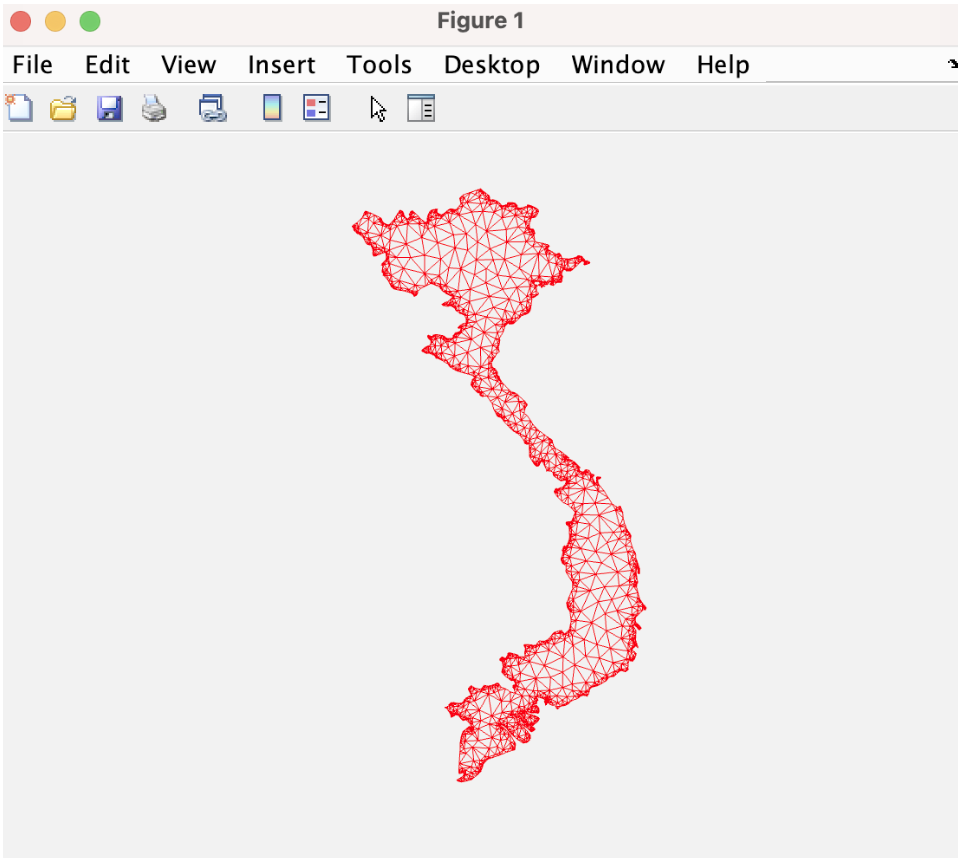
\includegraphics[width=\textwidth]{images/vietnam.png} 
        \caption{Visualization of Vietnam} 
        \label{fig:first}
    \end{subfigure}
    \hfill
    \begin{subfigure}[b]{0.4\textwidth}
        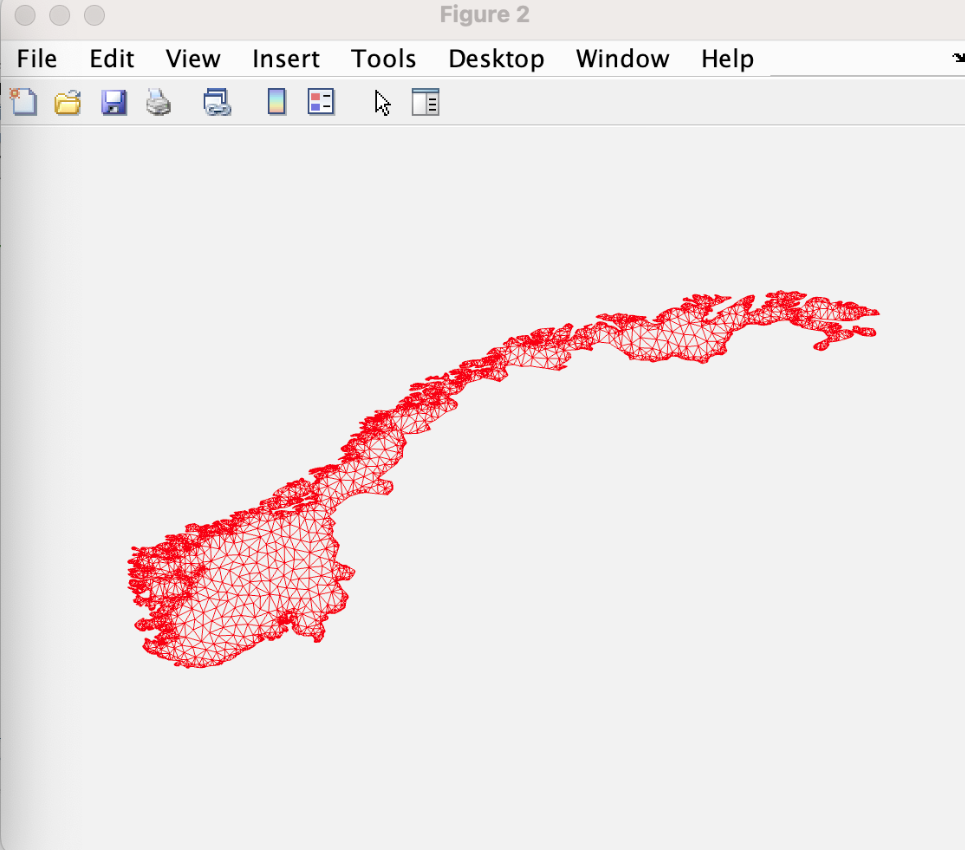
\includegraphics[width=\textwidth]{images/Norway.png} 
        \caption{Visualization of Norway} 
    \end{subfigure}
    
\end{figure}

\section{Task: Implement various graph partitioning algorithms [25 points]}


\begin{itemize}

\item Run in Matlab the script \texttt{Bench\_bisection.m} and familiarize yourself with the Matlab codes in the directory \texttt{Part\_Toolbox}. An overview of all functions and scripts is offered in \texttt{Contents.m}. 

\item Implement \textbf{spectral graph bisection} based on the entries of the Fiedler eigenvector. Use the incomplete Matlab file \texttt{bisection\_spectral.m} for your solution.

\item Implement \textbf{inertial graph bisection}. For a graph with 2D coordinates, this inertial bisection constructs a line such that half the nodes are on one side of the line, and half are on the other.
Use the incomplete Matlab file \texttt{bisection\_inertial.m} for your solution.
 
\item Report the bisection edgecut for all toy meshes that are either generated or loaded in the script \\ "Bench\_bisection.m." Use Table~\ref{table:bisection} to report these results.

\begin{table}[h]
\caption{Bisection results}
\centering
\begin{tabular}{l|r|r|r|r} \hline\hline 
Mesh             &  Coordinate           & Metis 5.0.2  & Spectral & Inertial  \\ \hline
mesh1e1          &   18                   &             &          &           \\             
mesh2e1          &   37                   &             &          &           \\ 
netz4504\_dual   &                        &             &          &           \\ 
stufe            &                        &             &          &           \\ 
\hline \hline
\end{tabular}
\label{table:bisection}
\end{table}

\end{itemize}

\begin{lstlisting}[language=MyMATLAB, style=mystyle, caption={Spectral Clustering and Bipartition}]
    [n,~] = size(xy);
    D_diag = diag(sum(A));
    L = D_diag - A;
    
    opts.sigma = 1e-10;
    opts.tol = 1e-10;
    [Vecs, Vals] = eigs(L, 2, 'smallestabs', opts);
    
    u2 = Vecs(:, 2);
    split = median(u2);
    
    a = find(u2 < split);
    b = find(u2 > split);
    c = find(u2 == split);
    
    nc = length(c);
    if nc
        na = length(a);
        nca = min(max(ceil(n/2) - na, 0), nc);
        a = [a; c(1:nca)];
        b = [b; c(nca+1:end)];
    end
    
    part1 = a';
    part2 = b';
\end{lstlisting}

\begin{lstlisting}[language=MyMATLAB, style=mystyle, caption={Computing Principal Direction and Partitioning Data}]
    x_mean = mean(xy(:,1));
    y_mean = mean(xy(:,2));
    
    S = cov(xy);           
    M = [S(2,2), S(1,2);   % S_xx and S_yy
         S(1,2), S(1,1)];  % S_xy
    
    [V, D] = eig(M);
    [~, ind] = min(diag(D));
    u = V(:,ind);
    u = [-u(1); u(2)];
    
    [part1, part2] = partition(xy, u);
\end{lstlisting}
The result of the bisection edgecut as following
\begin{table}[htbp]
    \centering
    \caption{Bisection results}
    \label{tab:bisection_results}
    \begin{tabular}{lcccc}
        \toprule
        \textbf{Mesh} & \textbf{Coordinate} & \textbf{Metis 5.0.2} & \textbf{Spectral} & \textbf{Inertial} \\
        \midrule
        mesh1e1          & 18  & 17  & 18  & 19  \\
        mesh2e1          & 37  & 37  & 35  & 47  \\
        mesh3e1          & 19  & 19  & 20  & 19  \\
        mesh3e5          & 19  & 19  & 24  & 19  \\
        airfoil1         & 94  & 77  & 132 & 94  \\
        netz4504\_dual   & 25  & 23  & 23  & 30  \\
        stufe            & 16  & 16  & 16  & 16  \\
        3elt             & 172 & 124 & 117 & 209 \\
        barth4           & 206 & 97  & 127 & 194 \\
        ukerbe1          & 32  & 27  & 36  & 28  \\
        crack            & 353 & 201 & 233 & 377 \\
        \bottomrule
    \end{tabular}
\end{table}
\section{Task: Recursively bisecting meshes [15 points]}

The recursive bisecion algorithm is implemented in the file \texttt{rec\_bisection.m} of the toolbox. Utilize this function within the script \texttt{Bench\_rec\_bisection.m} to recursively bisect the finite element meshes loaded within the script in 8 and 16 subgraphs. Use your inertial and spectral partitioning implementations, as well as the coordinate partitioning and the METIS bisection routine. Summarize your results in~\ref{table:Rec_bisection}. Finally, visualize the results for $p= 16$ for the case "crack".

\begin{table}[h]
\caption{Edge-cut results for recursive bi-partitioning.}
\centering
\begin{tabular}{l|r|r|r|r|r} \hline\hline 
 Case            &  Spectral             &  Metis 5.0.2    & Coordinate & Inertial  \\ \hline
 mesh3e1         &                       &                 &            &           \\             
 airfoil1        &                       &                 &            &           \\ 
 3elt            &                       &                 &            &           \\ 
 barth4          &                       &                 &            &           \\ 
 crack           &                       &                 &            &           \\ \hline \hline
\end{tabular}
\label{table:Rec_bisection}
\end{table}

The results of the edge cut are shown as following 
\begin{table}[htbp]
    \centering
    \caption{Edge-cut results for recursive 8-partitioning.}
    \label{tab:edgecut_8partitioning}
    \begin{tabular}{lcccc}
        \toprule
        \textbf{Case} & \textbf{Spectral} & \textbf{Metis 5.0.2} & \textbf{Coordinate} & \textbf{Inertial} \\
        \midrule
        airfoil1         & 398 & 320 & 516  & 578  \\
        netz4504\_dual   & 111 & 110 & 127  & 123  \\
        stufe            & 128 & 107 & 123  & 136  \\
        3elt             & 469 & 395 & 733  & 880  \\
        barth4           & 550 & 405 & 875  & 888  \\
        ukerbe1          & 128 & 128 & 225  & 281  \\
        crack            & 883 & 784 & 1343 & 1061 \\
        \bottomrule
    \end{tabular}
\end{table}


\begin{table}[htbp]
    \centering
    \caption{Edge-cut results for recursive 16-partitioning.}
    \label{tab:edgecut_16partitioning}
    \begin{tabular}{lcccc}
        \toprule
        \textbf{Case} & \textbf{Spectral} & \textbf{Metis 5.0.2} & \textbf{Coordinate} & \textbf{Inertial} \\
        \midrule
        airfoil1         & 633 & 563 & 819  & 903  \\
        netz4504\_dual   & 184 & 161 & 198  & 202  \\
        stufe            & 243 & 194 & 227  & 267  \\
        3elt             & 752 & 651 & 1168 & 1342 \\
        barth4           & 841 & 689 & 1306 & 1348 \\
        ukerbe1          & 224 & 224 & 374  & 470  \\
        crack            & 1419 & 1290 & 1860 & 1618 \\
        \bottomrule
    \end{tabular}
\end{table}
rec\_bisection is a function that recursively partitions a graph. It requires specifying different partitioning methods. There are four types of bisection\_spectral, bisection\_metis, bisection\_coordinate, and bisection\_inertial. For each method, 8 and 16 partitions need to be considered. For the visualization part, following is an example
\begin{lstlisting}[language=MyMATLAB, style=mystyle, caption={Recursive Bisection with Spectral Partitioning}]
    [map_spe8, sepij_spe8, sepA_spe8] = rec_bisection('bisection_spectral', 3, W, coords, 0);
\end{lstlisting}
\begin{figure}[htbp]
    \centering
    
    \begin{subfigure}[b]{0.3\textwidth}
        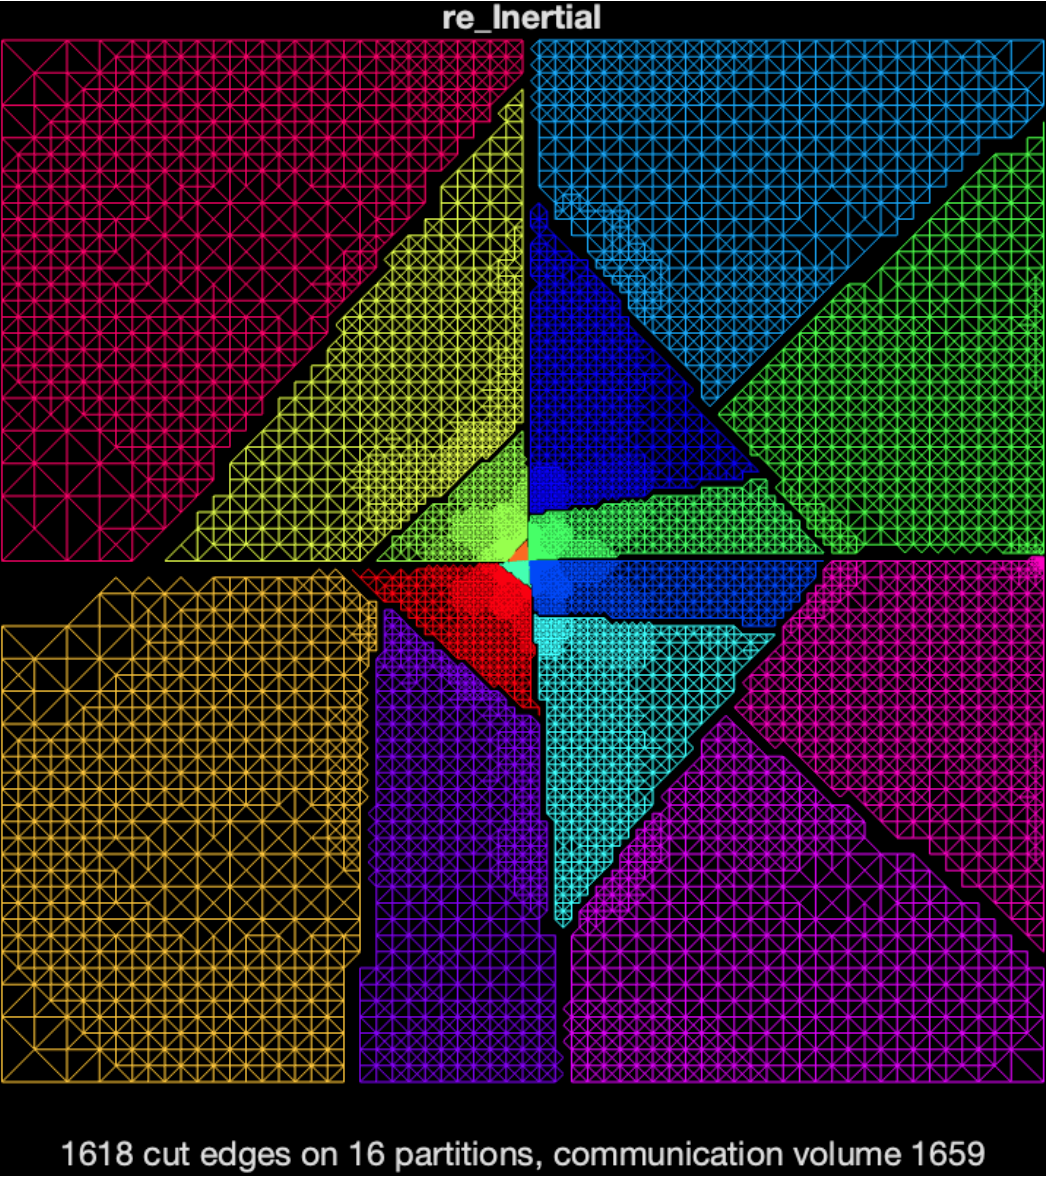
\includegraphics[width=\textwidth]{images/inertial.png}
        \caption{Visualization of inertial method}
    \end{subfigure}
    \hfill
    \begin{subfigure}[b]{0.3\textwidth}
        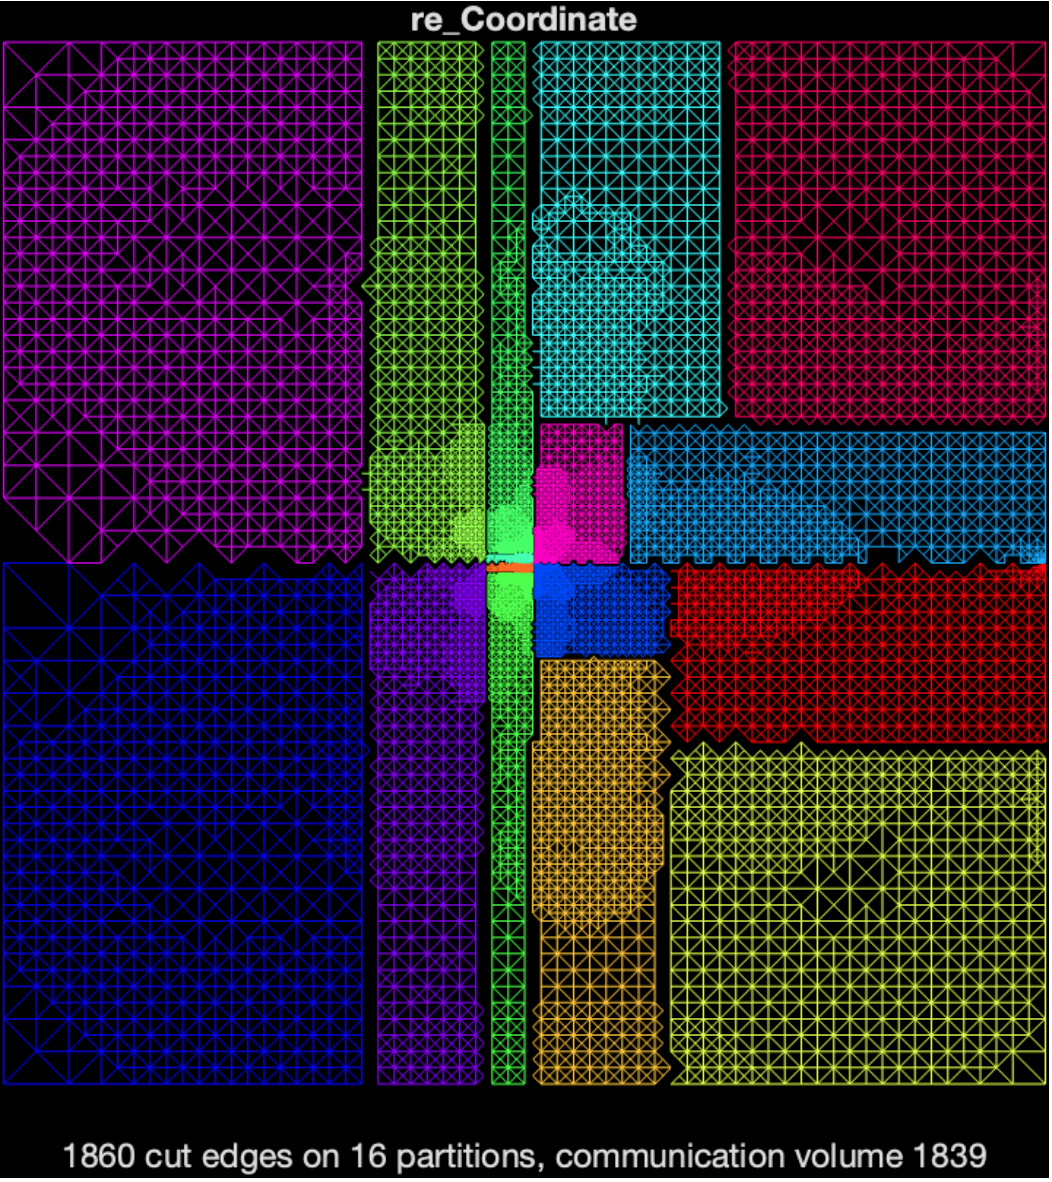
\includegraphics[width=\textwidth]{images/coordinate.png}
        \caption{Visualization of coordinate method} 
    \end{subfigure}
    
\end{figure}
\begin{figure}[htbp]
    \centering
    
    \begin{subfigure}[b]{0.3\textwidth}
        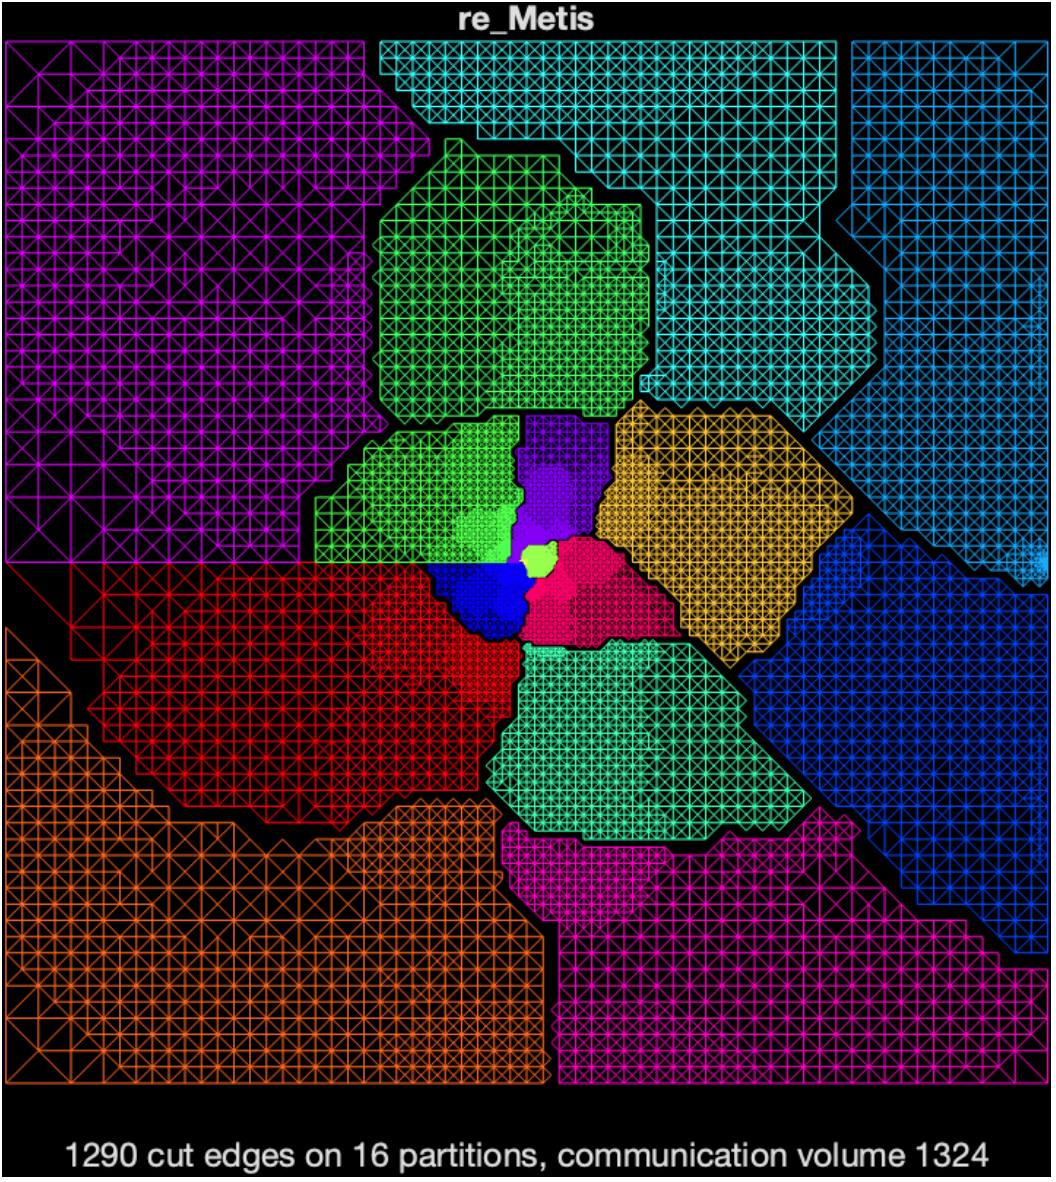
\includegraphics[width=\textwidth]{images/metis.png}
        \caption{Visualization of metis method}
    \end{subfigure}
    \hfill
    \begin{subfigure}[b]{0.3\textwidth}
        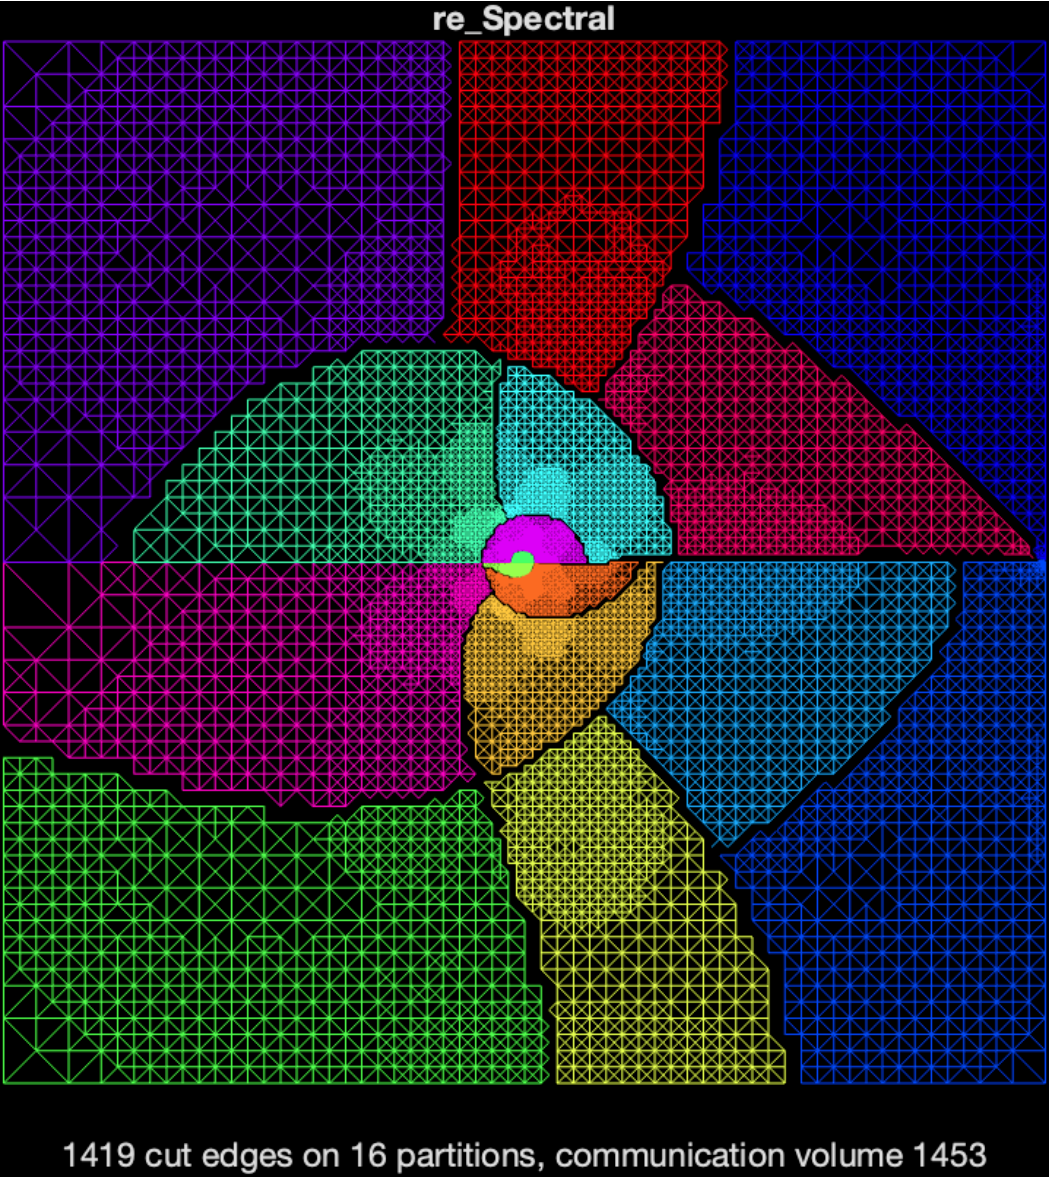
\includegraphics[width=\textwidth]{images/spectral.png}
        \caption{Visualization of spectral method} 
    \end{subfigure}
    
\end{figure}


\section{Task: Comparing recursive bisection to direct $k$-way partitioning [10 points]}

Use the incomplete \texttt{Bench\_metis.m} for your implementation. Compare the cut obtained from Metis 5.0.2 after applying recursive bisection and direct multiway partitioning for the graphs in question. Consult the Metis manual, and type \texttt{help metismex} in your MATLAB command line to familiarize yourself with the way the Metis recursive and direct multiway partitioning functionalities should be invoked. Summarize your results in Table~\ref{table:Compare_Metis} for 16 and 32 partitions. Comment on your results. Was this behavior anticipated? Visualize the partitioning results for both graphs for 32 partitions.

\begin{table}[h]
\caption{Comparing the number of cut edges for recursive bisection and direct multiway partitioning in Metis 5.0.2.}
\centering
\begin{tabular}{l|r|r|r|r|r|r|r|r} \hline\hline 
Partitions       &   Luxemburg           & usroads-48 &  Greece &  Switzerland &  Vietnam  &  Norway &  Russia  \\ \hline
 16              &                       &            &         &              &           &         &          \\             
 32              &                       &            &         &              &           &         &          \\ \hline \hline
\end{tabular}              
\label{table:Compare_Metis}
\end{table}

% -------------------------------------------------------------------------- %
% -------------------------------------------------------------------------- %
% --- Exercise 5 ----------------------------------------------------------- %
% -------------------------------------------------------------------------- %
% -------------------------------------------------------------------------- %
\begin{table}[htbp]
    \centering
    \caption{The number of cut edges for recursive bisection}
    \label{tab:recursive_bisection}
    \begin{tabular}{lccccccc}
        \toprule
        \textbf{Partitions} & \textbf{Luxemburg} & \textbf{usroads-48} & \textbf{Greece} & \textbf{Switzerland} & \textbf{Vietnam} & \textbf{Norway} & \textbf{Russia} \\
        \midrule
        16 & 197 & 607 & 297 & 730 & 245 & 284 & 616 \\
        32 & 322 & 988 & 509 & 1089 & 445 & 470 & 1006 \\
        \bottomrule
    \end{tabular}
\end{table}

\begin{table}[htbp]
    \centering
    \caption{The number of cut edges for direct multiway partitioning in Metis 5.0.2}
    \label{tab:multiway_partitioning}
    \begin{tabular}{lccccccc}
        \toprule
        \textbf{Partitions} & \textbf{Luxemburg} & \textbf{usroads-48} & \textbf{Greece} & \textbf{Switzerland} & \textbf{Vietnam} & \textbf{Norway} & \textbf{Russia} \\
        \midrule
        16 & 170 & 579 & 278 & 673 & 245 & 255 & 551 \\
        32 & 279 & 961 & 471 & 1042 & 411 & 439 & 933 \\
        \bottomrule
    \end{tabular}
\end{table}
The behavior of the direct k-section method corresponds to what we anticipated, that its result is better than the recursive method.
\begin{figure}[htbp]
    \centering
    
    \begin{subfigure}[b]{0.4\textwidth}
        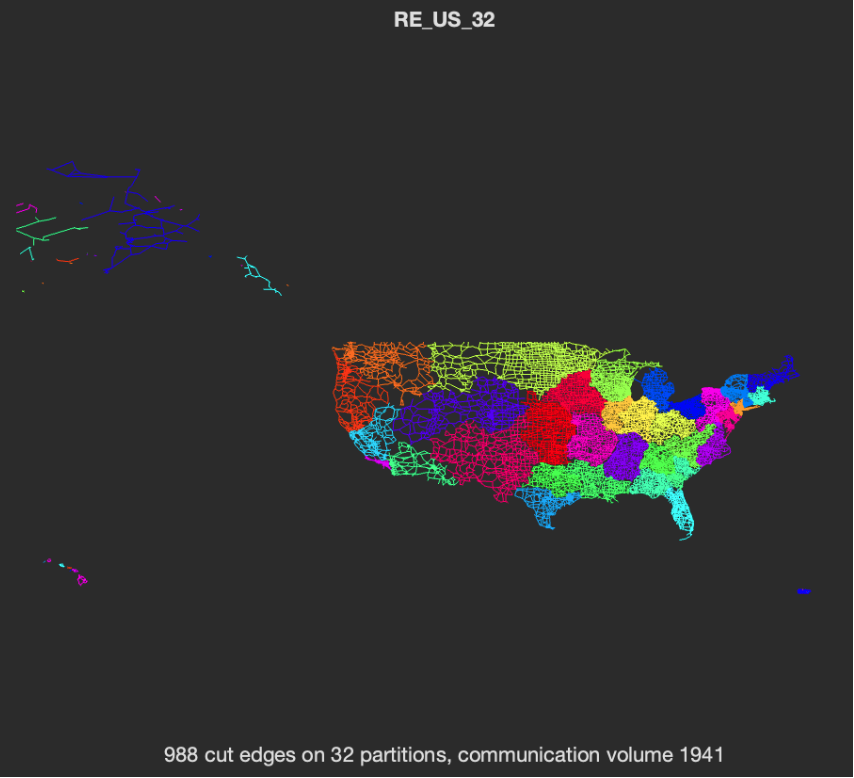
\includegraphics[width=\textwidth]{images/us-recu.png}
        \caption{Visualization of US-recursive}
    \end{subfigure}
    \hfill
    \begin{subfigure}[b]{0.4\textwidth}
        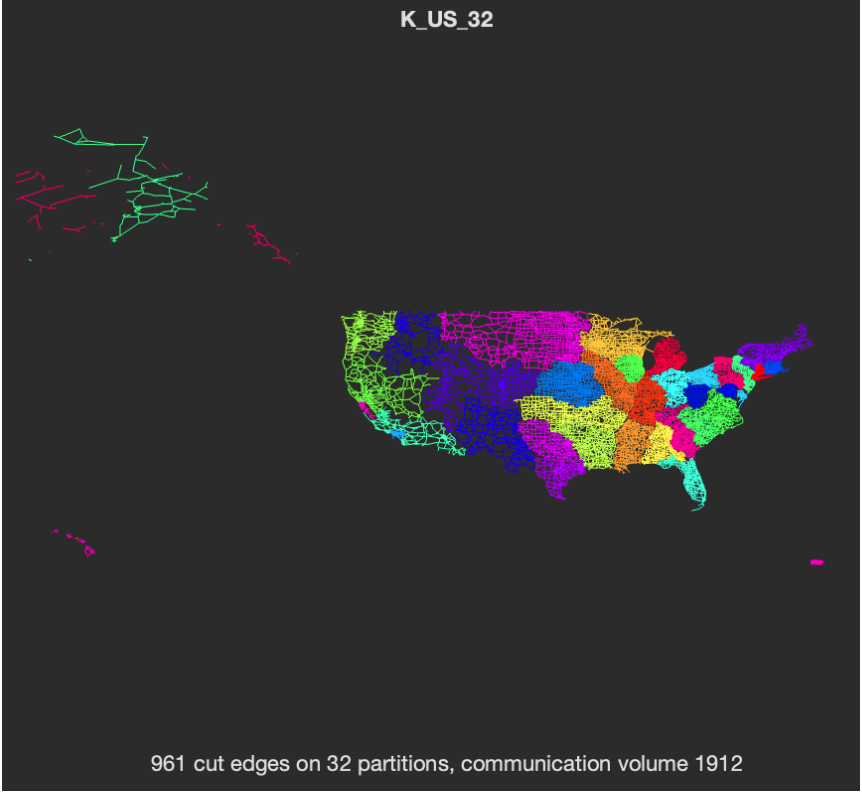
\includegraphics[width=\textwidth]{images/us-kway.png}
        \caption{Visualization of US-kway} 
    \end{subfigure}
    
\end{figure}

\begin{figure}[htbp]
    \centering
    
    \begin{subfigure}[b]{0.4\textwidth}
        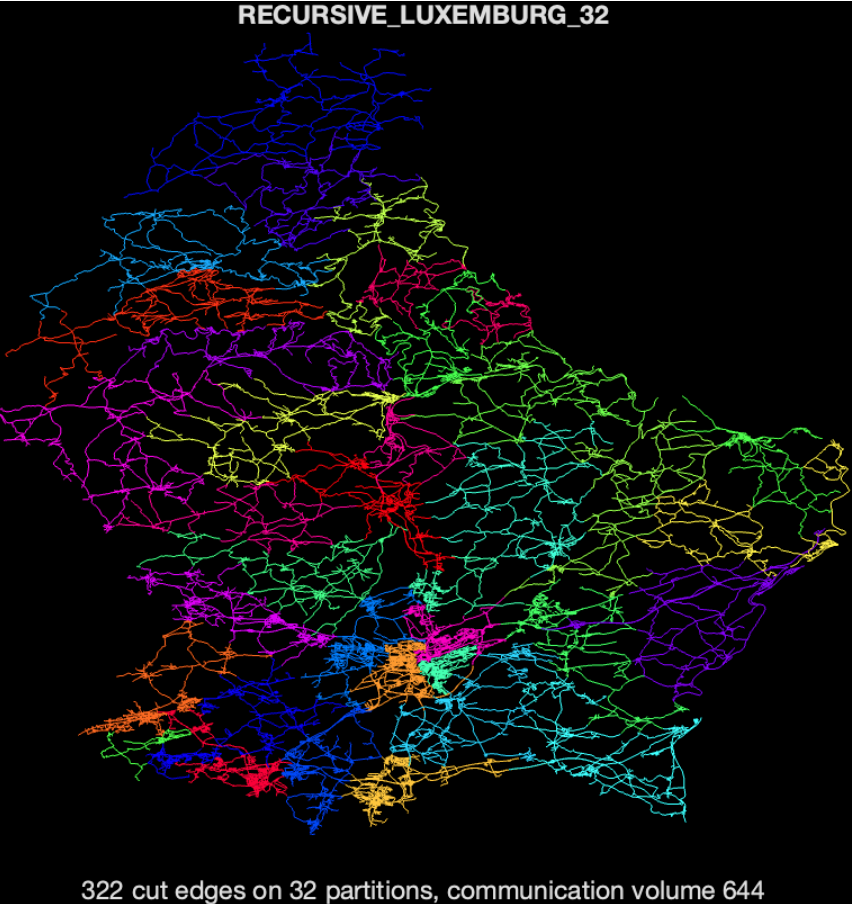
\includegraphics[width=\textwidth]{images/lu-recu.png}
        \caption{Visualization of LU-recursive}
    \end{subfigure}
    \hfill
    \begin{subfigure}[b]{0.4\textwidth}
        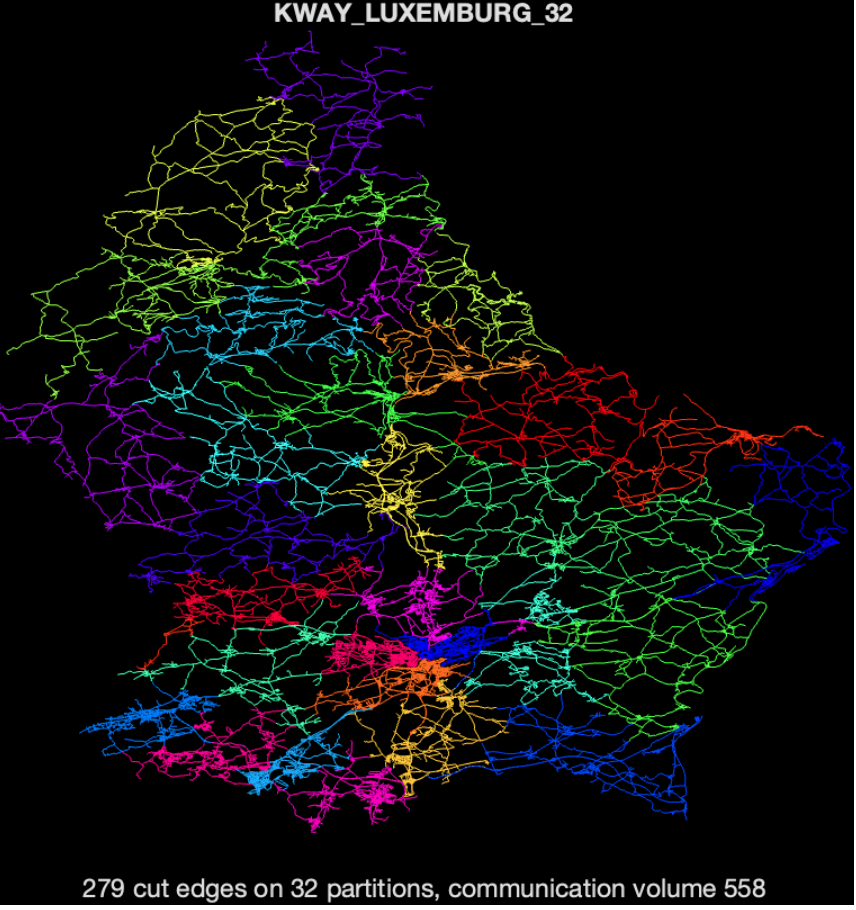
\includegraphics[width=\textwidth]{images/lu-kway.png}
        \caption{Visualization of LU-kway} 
    \end{subfigure}
    
\end{figure}

\begin{figure}[htbp]
    \centering
    
    \begin{subfigure}[b]{0.4\textwidth}
        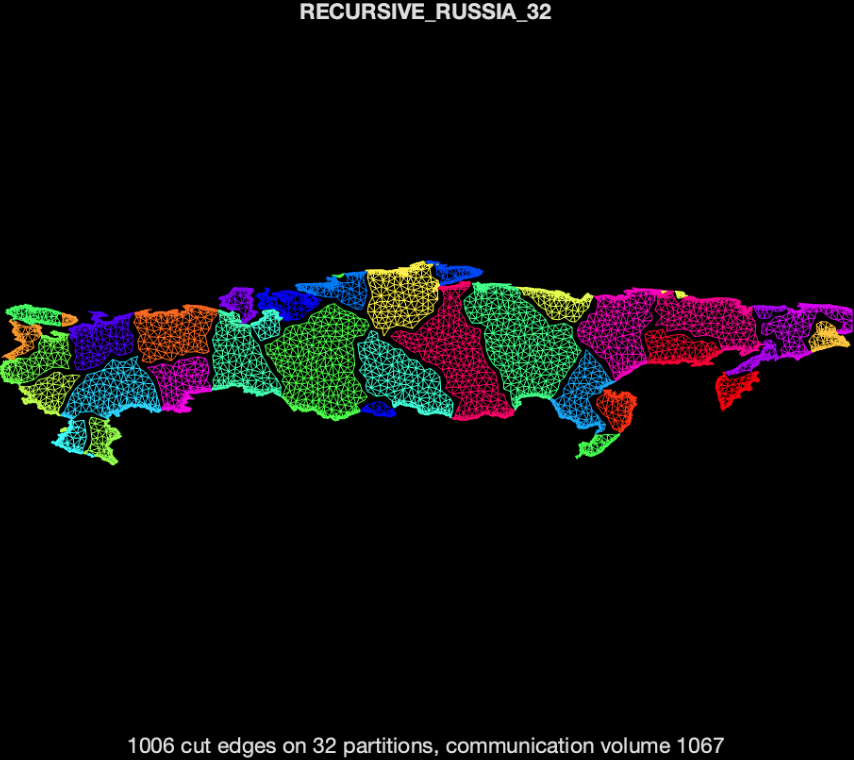
\includegraphics[width=\textwidth]{images/ru-recu.png}
        \caption{Visualization of RU-recursive}
    \end{subfigure}
    \hfill
    \begin{subfigure}[b]{0.4\textwidth}
        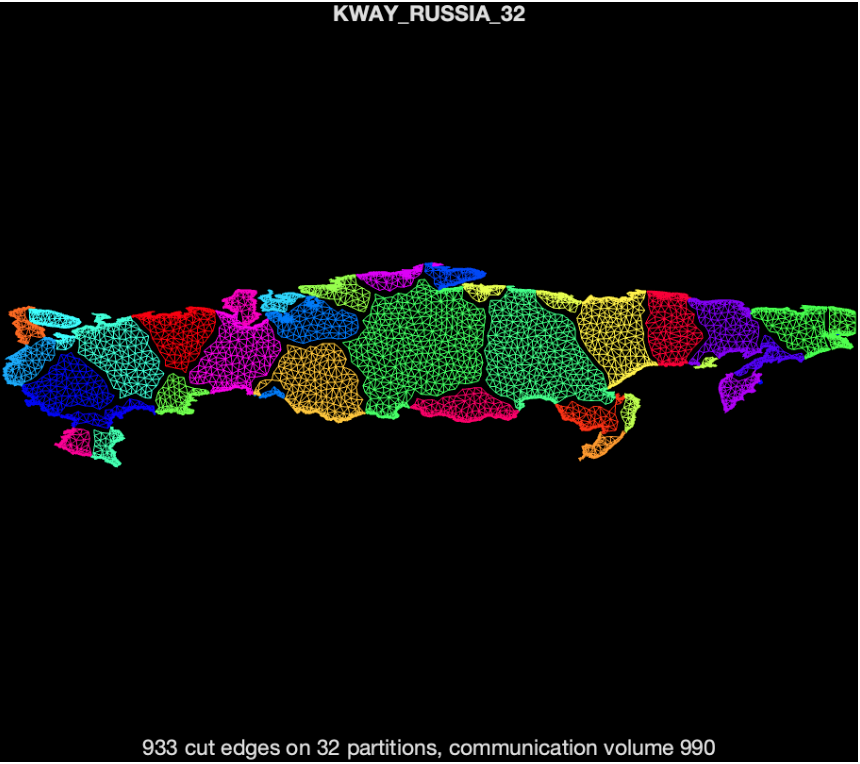
\includegraphics[width=\textwidth]{images/ru-kway.png}
        \caption{Visualization of RU-kway} 
    \end{subfigure}
    
\end{figure}

\section{Task: Utilizing graph eigenvectors [25 points]}


Provide the following illustrative results. Use the incomplete script \texttt{Bench\_eigen\_plot.m} for your implementation.

\begin{figure}[!t]
	\begin{center}
		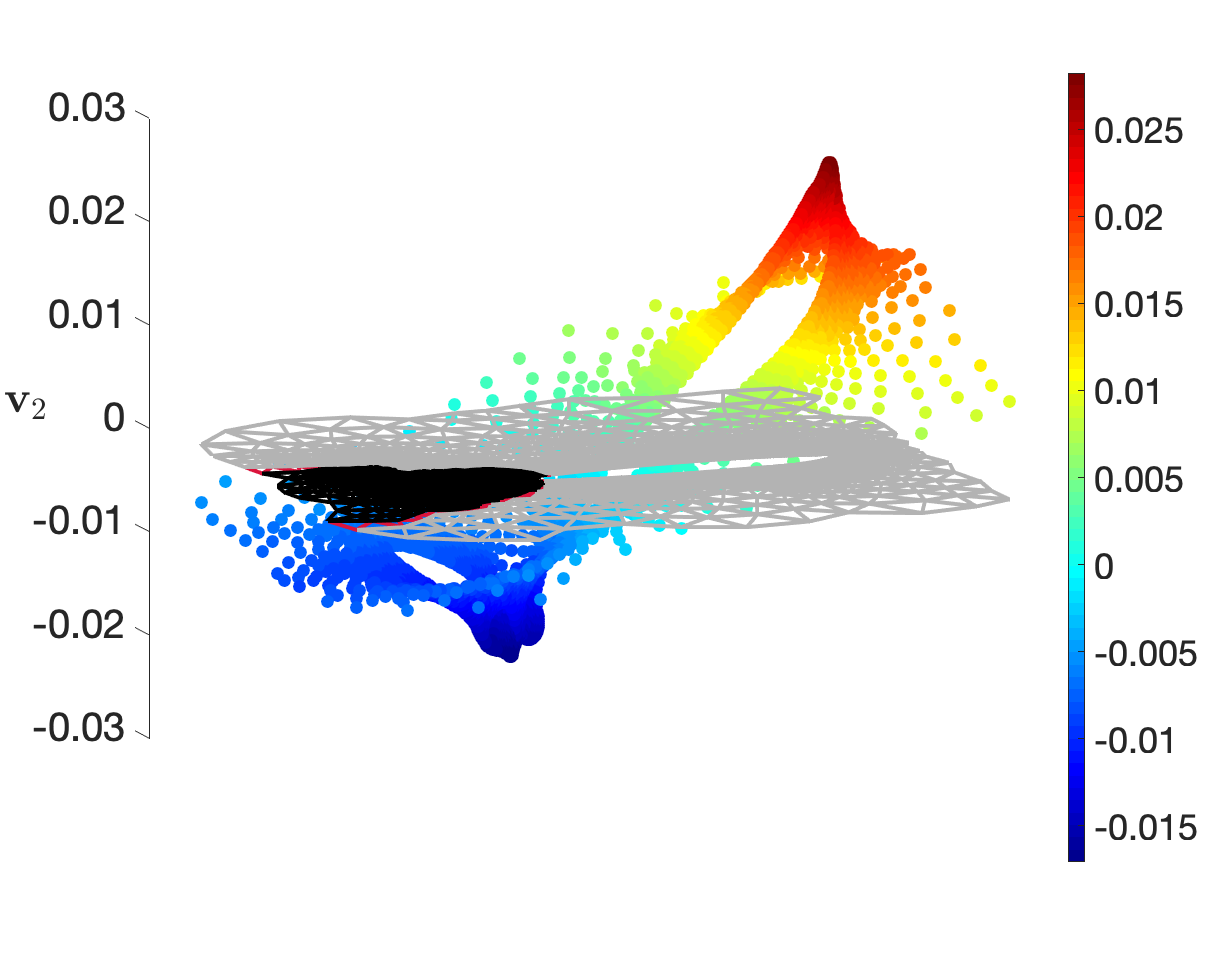
\includegraphics[width=0.55\textwidth]{images/fiedler_airfoil.png}
		\caption{Partitioning the Airfoil graph based on the values of the Fiedler eigenvector. The two partitions are depicted in black and gray, while the cut edges in red respectively. The z-axis represents the value of the entries of the eigenvector.}
		 \label{fig:fiedler_airfoil}
	\end{center}
\end{figure}


\begin{enumerate}
    \item Plot the entries of the eigenvectors associated with the first ($\lambda_1$) and second ($\lambda_2$)  smallest eigenvalues of the graph Laplacian matrix $\mathbf{L}$ for the graph "airfoil1." Comment on the visual result. Is this behavior expected?
    \item Plot the entries of the eigenvector associated with the second smallest eigenvalue $\lambda_2$ of the Graph Laplacian matrix $\mathbf{L}$. Project each solution on the coordinate system space of the following graphs: mesh3e1, barth4, 3elt, crack. An example is shown in Figure~\ref{fig:fiedler_airfoil}, for the graph "airfoil1". \newline
    \textbf{Hint}: You might have to modify the functions \texttt{gplotg.m} and \texttt{gplotpart.m} to get the desired result.
    \item In this assignment we dealt exclusively with graphs $\mathcal{G}(V,E)$ that have coordinates associated with their nodes. This is, however, most commonly not the case when dealing with graphs, as they are in fact abstract structures, used for describing the relation $E$ over a collection of entities $V$. These entities very often cannot be described in a Euclidean coordinate space. Therefore graph drawing is a tool to visualize relational information between nodes. The optimality of graph drawing is measured in terms of computation speed the ultimate usefulness of the resulting layout~\cite{Koren05}. A successful layout should transmit the clearly the desired message, e.g the subsets of a partitioned graph.
    We will now see a spectral graph drawing method, which constructs the layout utilizing the eigenvectors of the graph Laplacian matrix $\mathbf{L}$. Draw the graphs mesh3e1, barth4, 3elt, crack, and their \textbf{spectral bi-partitioning} results using the eigenvectors to supply coordinates. Locate vertex $i$ at position:
    \begin{equation*}
        x_i = \left( \mathbf{v}_2(i), \mathbf{v}_3(i) 
        \right),
    \end{equation*}
    where $\mathbf{v}_2, \mathbf{v}_3$ are the eigenvectors associated with the 2nd and 3rd smallest eigenvalues of $\mathbf{L}$. Figure~\ref{fig:spectral_layout} illustrates these 2 ways of visualizing the partitions of the  "airfoil1" graph.
\end{enumerate}


\begin{figure}[!h]
\begin{center}
  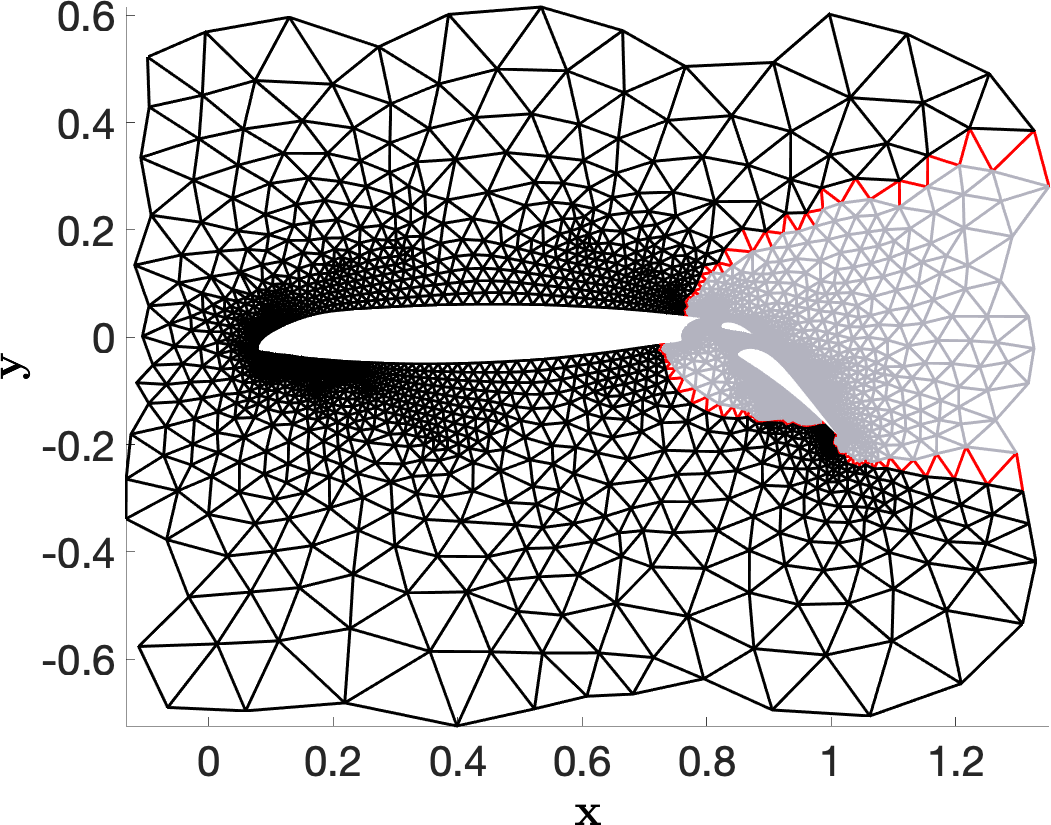
\includegraphics[width=0.35\textwidth]{images/airfoil_part_spat.png}
  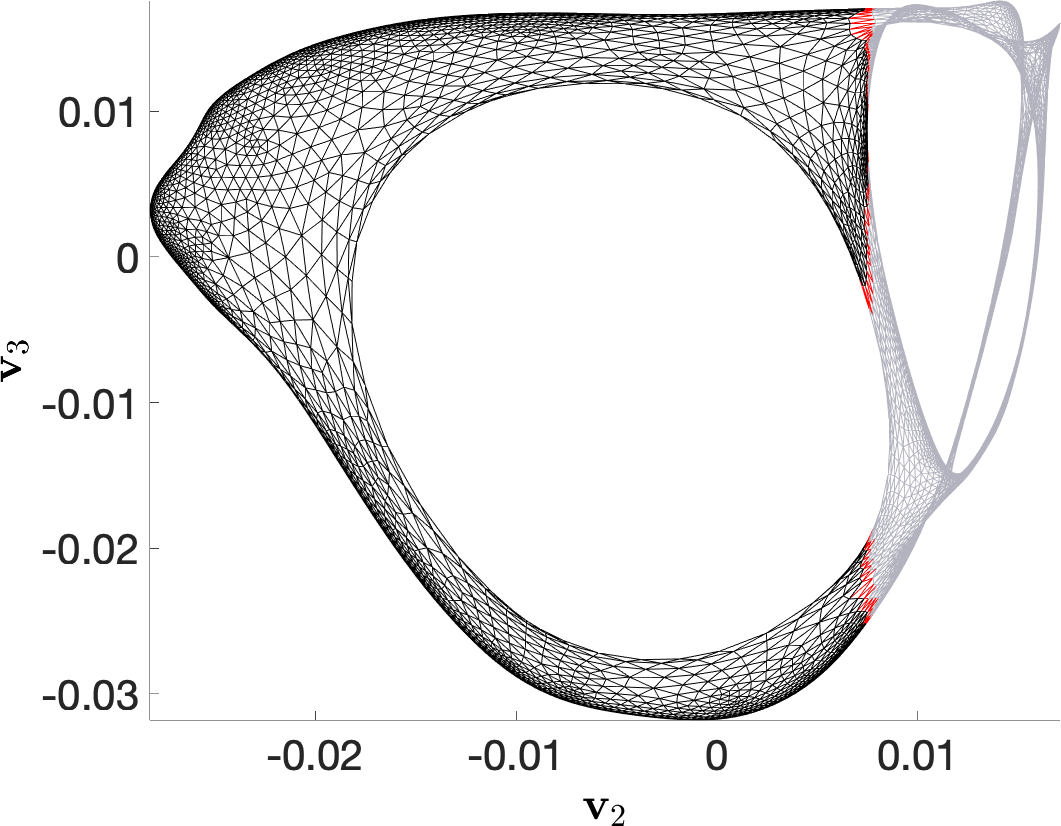
\includegraphics[width=0.35\textwidth]{images/airfoil_part_spec.png}
  \caption{Visualizing the bipartitioning of the graph "airfoil1" with 4253 nodes and 12289 edges. Left: Spatial coordinates. Right: Spectral coordinates.}
  \label{fig:spectral_layout}
\end{center}
\end{figure}

It is predicted that partitions based on the second smallest eigenvalue perform better than those based on the smallest eigenvalue.
\begin{figure}[htbp]
    \centering
    
    \begin{subfigure}[b]{0.4\textwidth}
        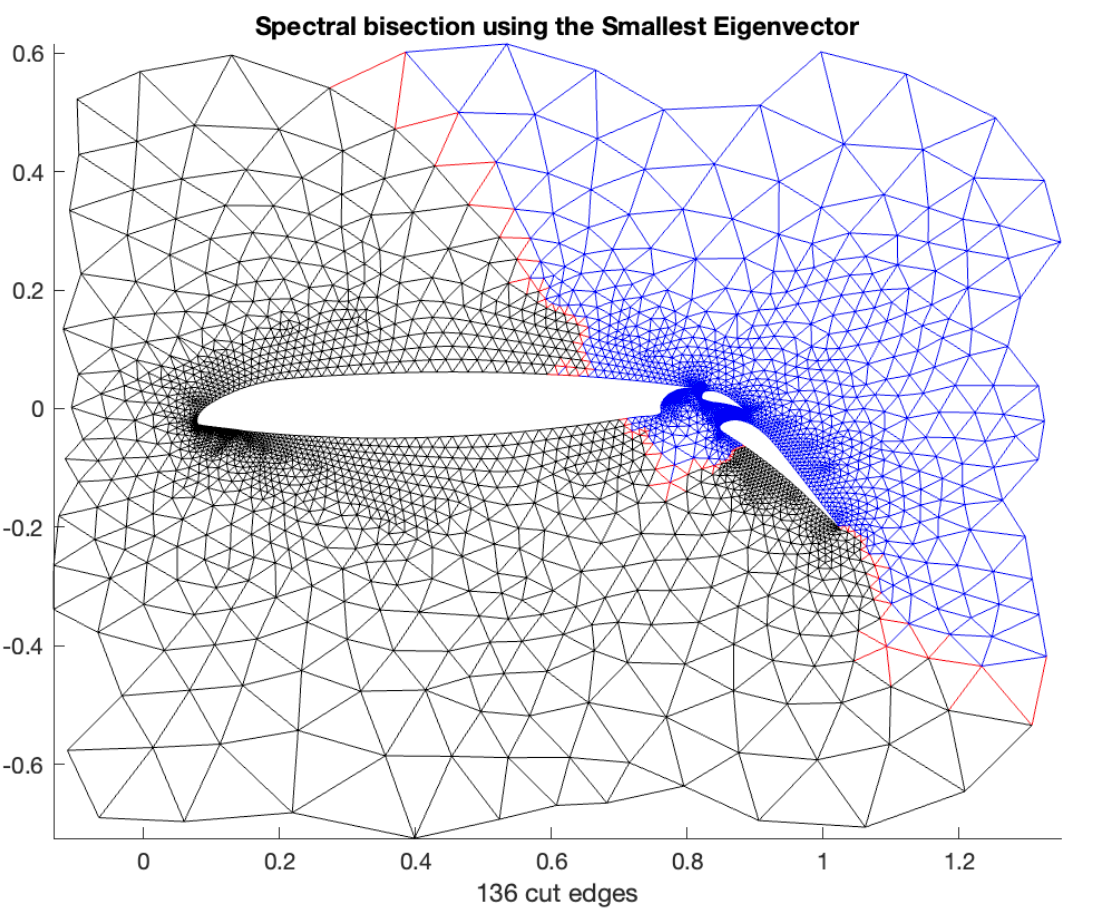
\includegraphics[width=\textwidth]{images/smallest eigenvalue.png}
        \caption{Smallest eigenvalue}
    \end{subfigure}
    \hfill
    \begin{subfigure}[b]{0.4\textwidth}
        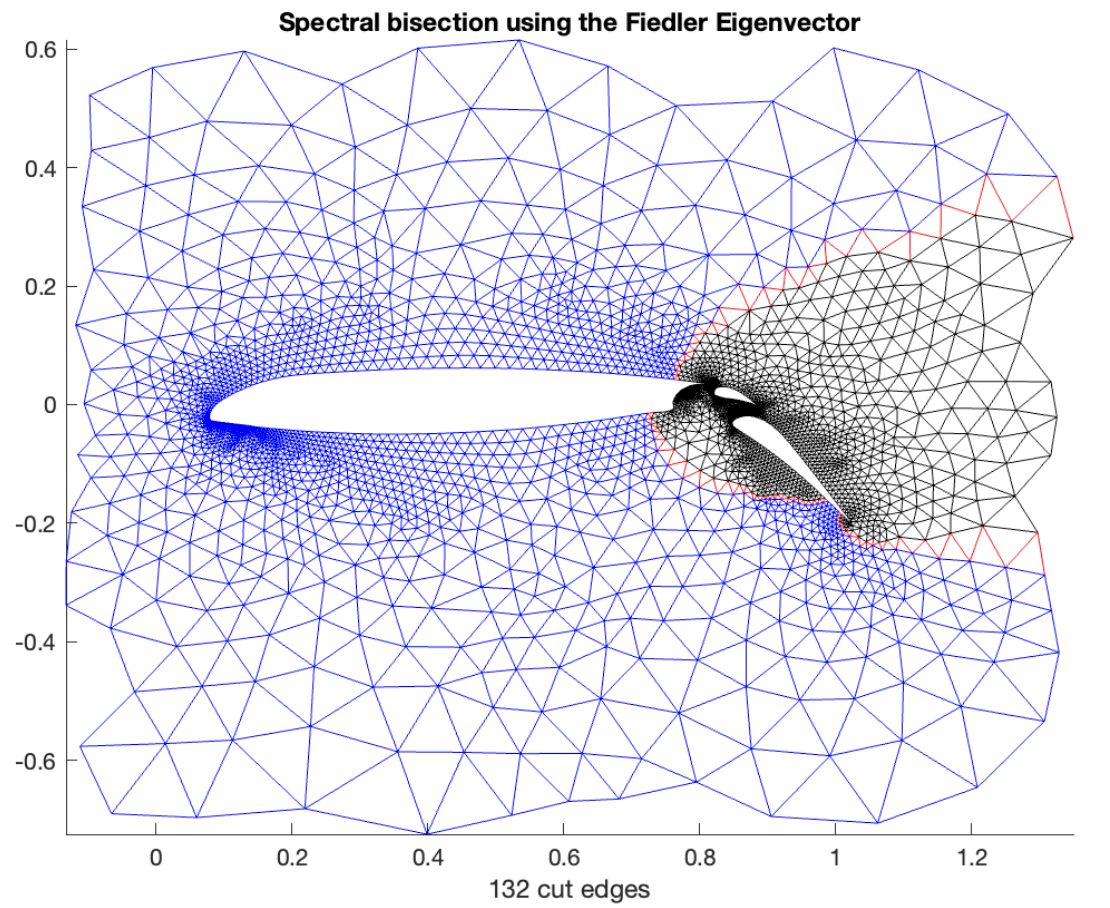
\includegraphics[width=\textwidth]{images/Secondsmallest.png}
        \caption{Second smallest eigenvalue} 
    \end{subfigure}
    
\end{figure}

\begin{figure}[htbp]
    \centering
    
    \begin{subfigure}[b]{0.4\textwidth}
        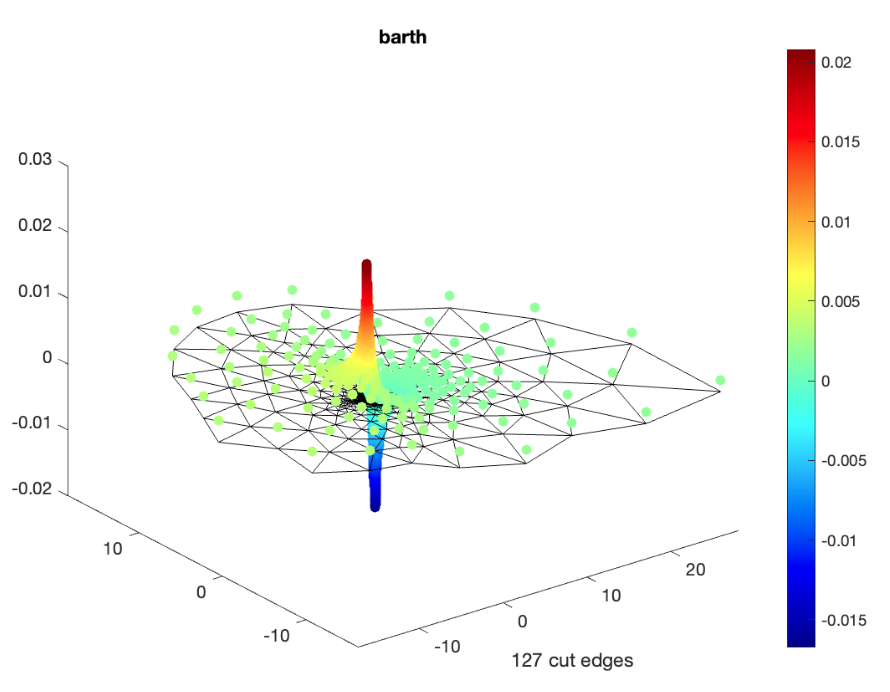
\includegraphics[width=\textwidth]{images/barth.png}
        \caption{barth}
    \end{subfigure}
    \hfill
    \begin{subfigure}[b]{0.4\textwidth}
        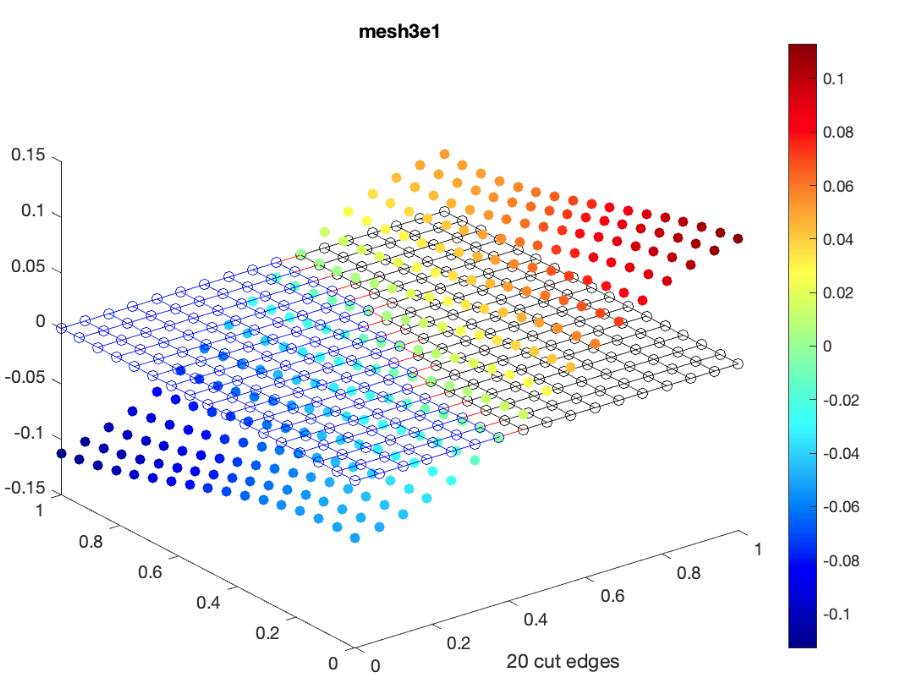
\includegraphics[width=\textwidth]{images/mesh3e1.png}
        \caption{mesh3e1} 
    \end{subfigure}
    
\end{figure}

\begin{figure}[htbp]
    \centering
    
    \begin{subfigure}[b]{0.4\textwidth}
        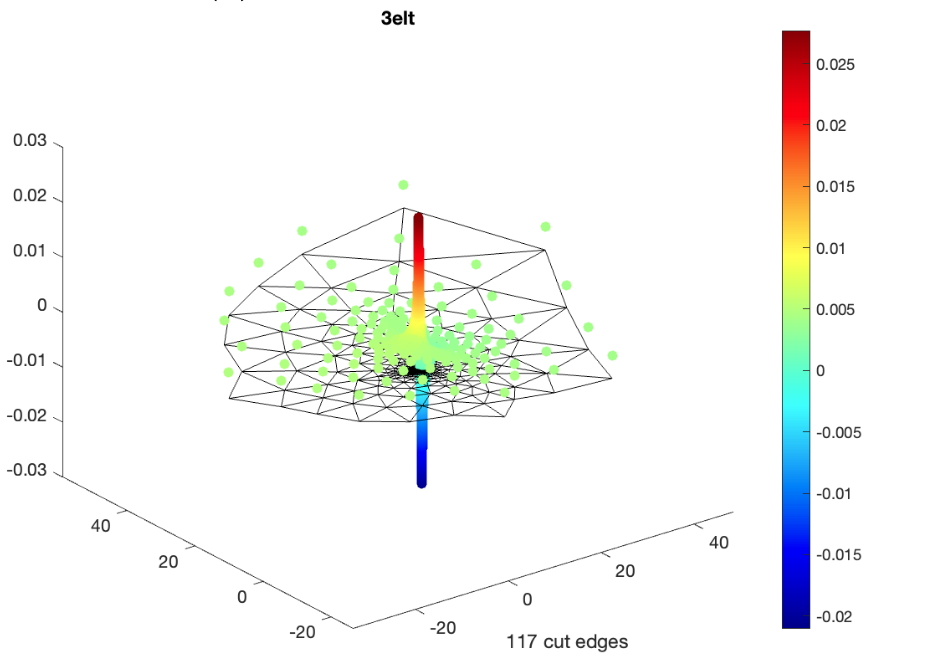
\includegraphics[width=\textwidth]{images/3elt.png}
        \caption{3elt}
    \end{subfigure}
    \hfill
    \begin{subfigure}[b]{0.4\textwidth}
        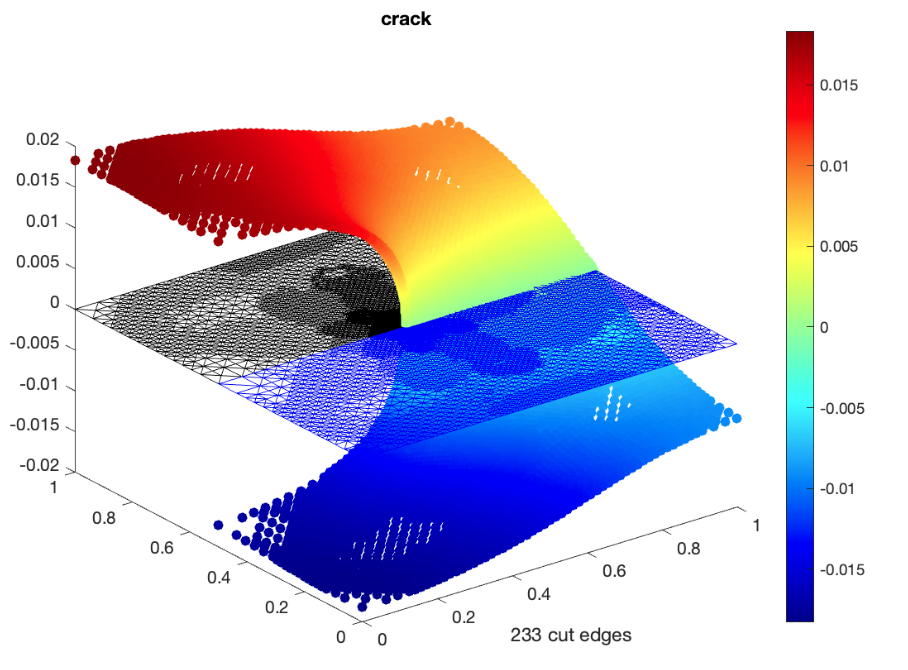
\includegraphics[width=\textwidth]{images/crack.png}
        \caption{crack} 
    \end{subfigure}
    
\end{figure}

\begin{figure}[htbp]
    \centering
    
    \begin{subfigure}[b]{0.4\textwidth}
        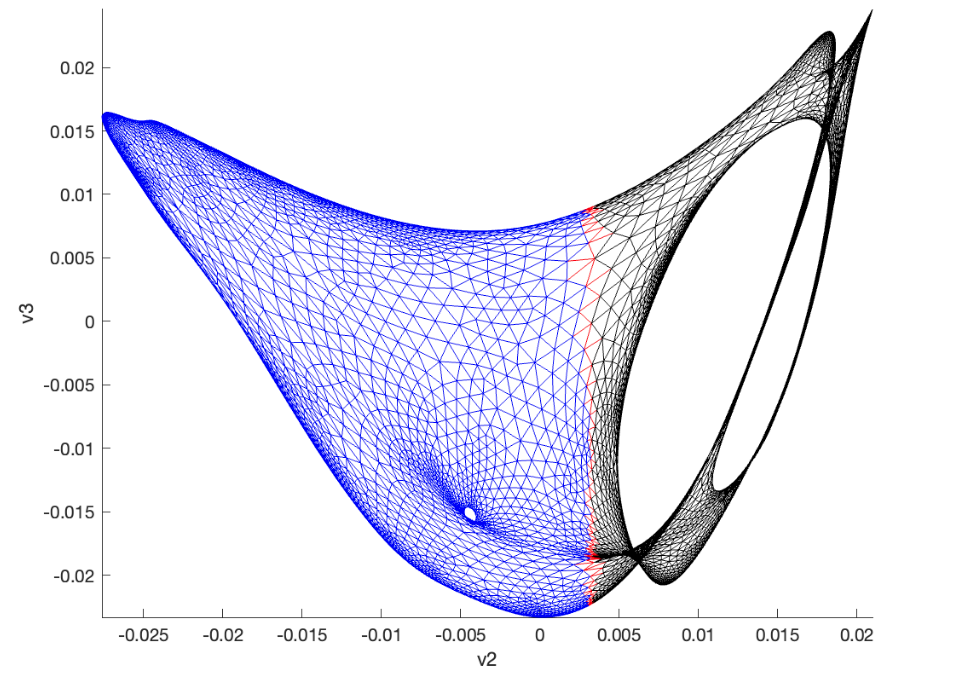
\includegraphics[width=\textwidth]{images/bi-3elt.png}
        \caption{bi-3elt}
    \end{subfigure}
    \hfill
    \begin{subfigure}[b]{0.4\textwidth}
        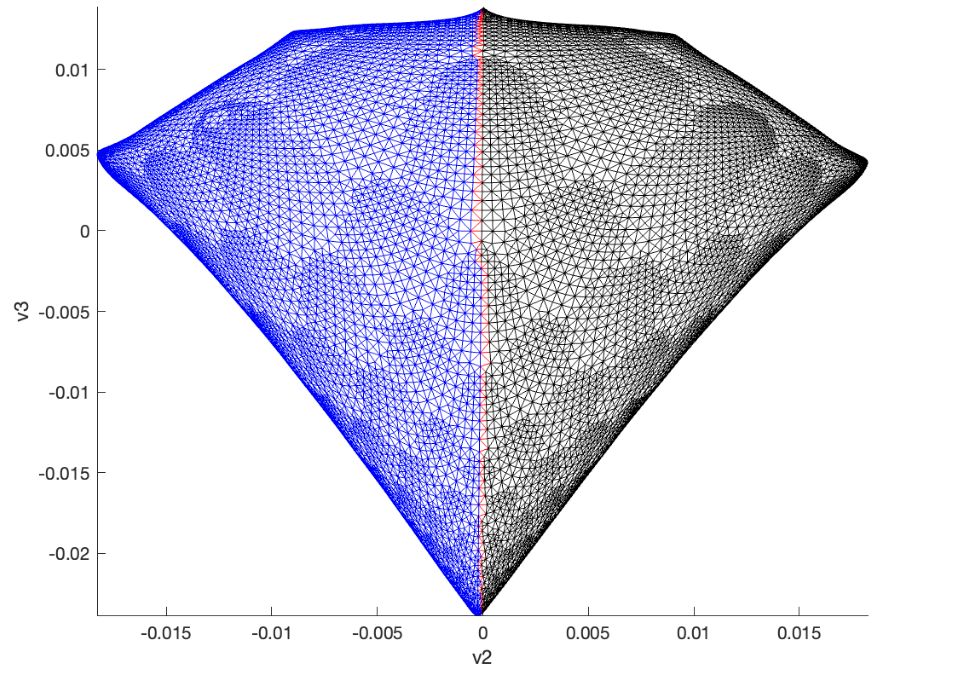
\includegraphics[width=\textwidth]{images/bi-crack.png}
        \caption{bi-crack} 
    \end{subfigure}
    
\end{figure}

\begin{figure}[htbp]
    \centering
    
    \begin{subfigure}[b]{0.4\textwidth}
        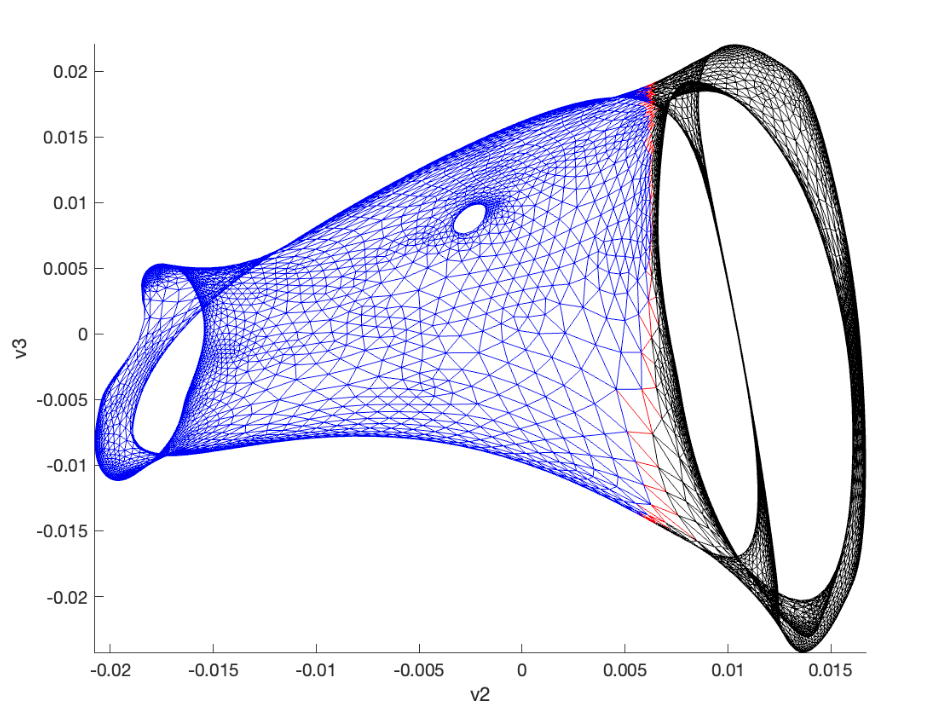
\includegraphics[width=\textwidth]{images/bi-barth.png}
        \caption{bi-barth}
    \end{subfigure}
    \hfill
    \begin{subfigure}[b]{0.4\textwidth}
        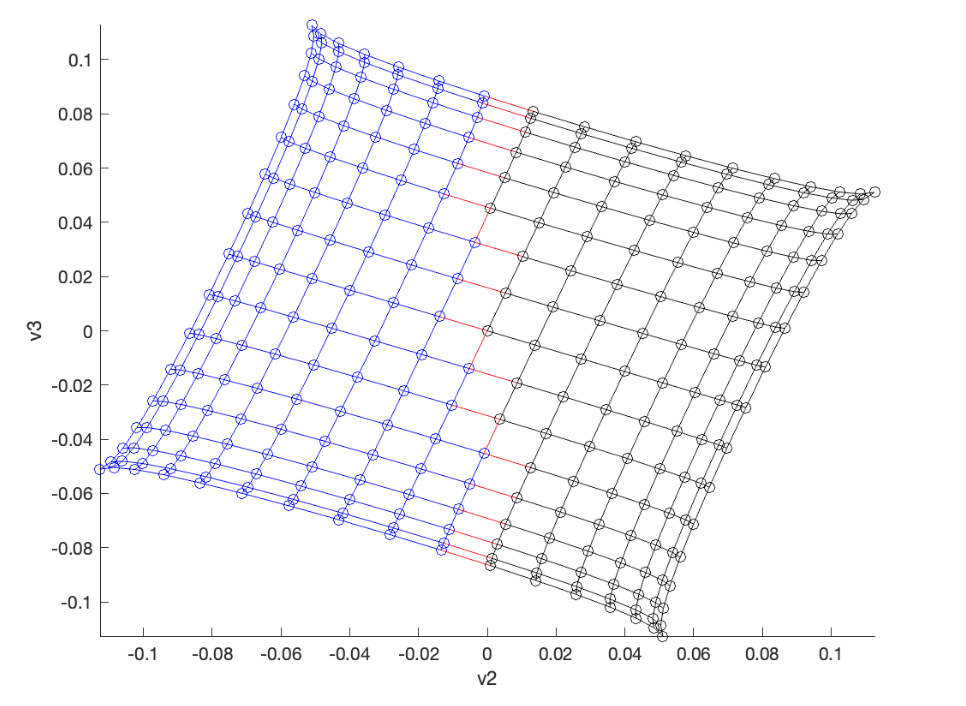
\includegraphics[width=\textwidth]{images/bi-mesh3e1.png}
        \caption{bi-mesh3e1} 
    \end{subfigure}
    
\end{figure}



\bibliographystyle{plain}
\bibliography{template}

% -------------------------------------------------------------------------- %
% -------------------------------------------------------------------------- %
% --- Report Quality ------------------------------------------------------- %
% -------------------------------------------------------------------------- %
% -------------------------------------------------------------------------- %




\section*{Additional notes and submission details}
Submit the source code files (together with your used \texttt{Makefile}) in
an archive file (tar, zip, etc.), and summarize your results and the
observations for all exercises by writing an extended Latex report.
Use the Latex template from the webpage and upload the Latex summary
as a PDF to \href{https://www.icorsi.ch}{iCorsi}.

\begin{itemize}
	\item Your submission should be a gzipped tar archive, formatted like project\_number\_lastname\_firstname.zip or project\_number\_lastname\_firstname.tgz. 
	It should contain:
	\begin{itemize}
		\item all the source codes of your MATLAB solutions;
		\item your write-up with your name  project\_number\_lastname\_firstname.pdf.
	\end{itemize}
	\item Submit your .zip/.tgz through Icorsi.
\end{itemize}

\end{document}
